\documentclass{beamer}

\usepackage{xltxtra}
\usepackage[lithuanian]{babel}
\usepackage{mathtools}
\usepackage{cite}
\usepackage{multimedia}

\title{Kompiuterinis difuzijos įtakos krūvininkų pernašai modeliavimas}

\author
{V. Valentinavičius}

\date{Vilnius, 2012}
\subject{Kursinis darbas}

\begin{document}
\frame{\titlepage}
  \begin{frame}
    \frametitle{Darbo tikslai}
    \begin{itemize}
      \item Skaitmeniškai modeliuojant nustatyti difuzijos įtaką krūvininkų pernašai photo-CELIV atveju, esant skirtingiems krūvininkų pradiniams pasiskirstymams.
      \item Nustatyti sąlygas, kurioms esant difuzija gali turėti įtakos krūvininkų rekombinacijos spartos matavimų rezultatus.
    \end{itemize}
  \end{frame}
  \begin{frame}
    \frametitle{Metodas}
    \begin{itemize}
	\item Naudota programa simuliuojanti bandinius, kuriuose pasireiškia difuzijos, dreifo ir rekombinacijos reiškiniai
	\item Programa leidžia atkartoti realaus eksperimento eigą ir sąlygas 
	\item Tirtas virtualaus bandinio elgesys simuliuojant photo-CELIV metodiką
	\item Rekombinacijos koeficientas matuotas iš photo-CELIV srovės kinetikos maksimumo priklausomybės nuo užlaikymo trukmės~\(t_{delay}\)
	\end{itemize}        
  \end{frame}
  \begin{frame}
    \frametitle{Parametrai}
    \begin{itemize}
    \item Pasirinkti pilnai blokuojantys bandinio kontaktai
	\item Krūvininkų judrių santykis \(\frac{\mu_n}{\mu_p} = 1000\)
	\item Bimolekulinė rekombinacija pagal Lanževeną \(B_L=\frac{e}{\varepsilon \varepsilon_0}(\mu_n+\mu_p)\)
	\item Difuzijos koeficientas suskaičiuojamas pagal Einšteino dėsnį \(D=\frac{k_B T \mu }{e}\)
	\end{itemize}
  \end{frame}
  \begin{frame}
    \frametitle{Svarbiausi darbo rezultatai ir išvados}
    \framesubtitle{Difuzijos įtaka krūvininkų judrio matavimams}
    \begin{figure}
    	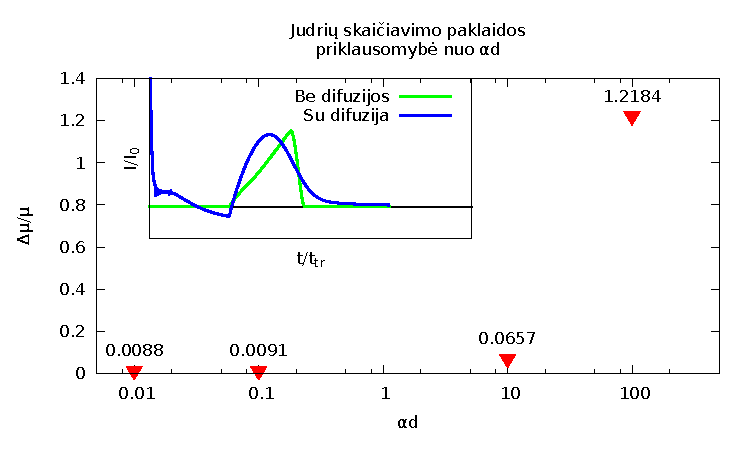
\includegraphics[width=0.9\textwidth]{./pdf/mu.pdf}
    \end{figure}
    \begin{itemize}
      \item Naudojant standartinę photo-CELIV formulę gaunama paklaida tarp judrio verčių su difuzija ir be jos siekia 120\%.
    \end{itemize}
  \end{frame}
  \begin{frame}
    \frametitle{Svarbiausi darbo rezultatai ir išvados}
    \framesubtitle{Difuzijos įtaka krūvininkų rekombinacijos matavimams}
    \begin{figure}
    	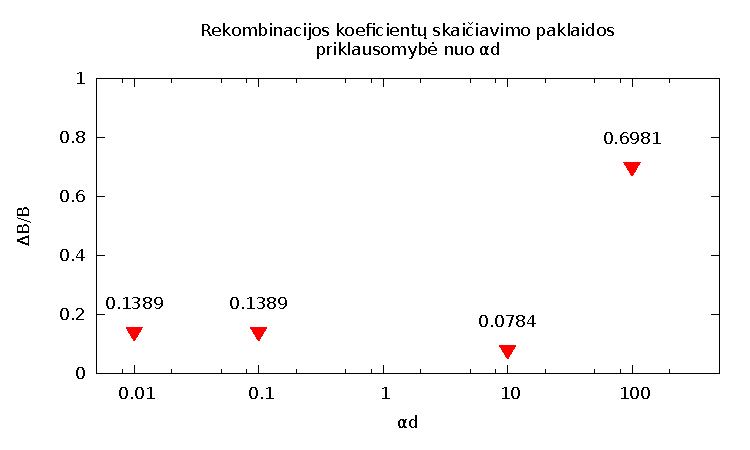
\includegraphics[width=0.9\textwidth]{./pdf/beta.pdf}
    \end{figure}
    \begin{itemize}
      \item Neatsižvelgus į difuzijos įtaką skaičiuojant rekombinacijos spartą, esant paviršinei sugerčiai \(\alpha d = 100\), galima padaryti paklaidą siekiančia 70\%.
    \end{itemize}
  \end{frame}
  
  \begin{frame}
    \frametitle{Svarbiausi darbo rezultatai ir išvados}
    \framesubtitle{Rekombinacijos tipas nekinta}
    \begin{figure}
    	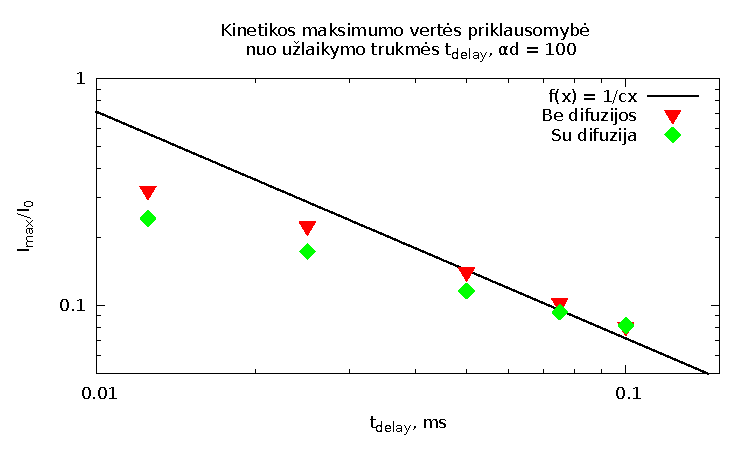
\includegraphics[width=0.9\textwidth]{./pdf/ad100_recomb.pdf}
    \end{figure}
    \begin{itemize}
      \item Dėl difuzijos įskaitymo rekombinacijos tipas nepakinta, net ir esant paviršinei sugerčiai (\(\alpha d = 100\)).
    \end{itemize}
  \end{frame}
  
  \begin{frame}
    \frametitle{Svarbiausi darbo rezultatai ir išvados}
    \framesubtitle{Atgalinė srovė photo-CELIV kinetikose}
    \begin{figure}
    	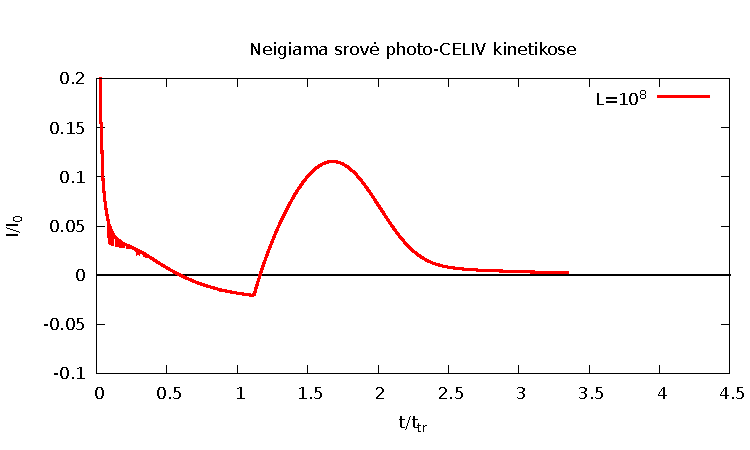
\includegraphics[width=0.9\textwidth]{./pdf/negative.pdf}
    \end{figure}
    \begin{itemize}
      \item Pastebėta atgalinė srovė tekanti esant paviršinei krūvininkų generacijai dar neįjungus CELIV įtampos signalo. Manoma, jog ji nepastebėta eksperimente dėl mažos vertės arba ją slepia kiti efektai.
    \end{itemize}
  \end{frame}
  
    \begin{frame}
    \frametitle{Planai}
    \begin{itemize}
      \item Ištirti atgalinės srovės atsiradimo priežastis ir stebėjimo ribas
      \item Įvesti krūvininkų prilipimo ir atlipimo reiškinius
      \item Patikrinti eksperimentų, kuriuose parodomas krūvininkų judrio mažėjimas nuo užlaikymo trukmės \(t_{delay}\), rezultatus teoriškai
    \end{itemize}
  \end{frame}
  
  \begin{frame}
  \frametitle{Pabaiga}
  Gal turite klausimų?
  \end{frame}
  
\end{document}